\chapter{Il progetto LHC:}


\section{Large Hadron Collider}
Formato da un anello di circonferenza pari a 27 km, il Large Hadron Collider (LHC), situato al CERN a Ginevra, Svizzera, è il più grande acceleratore di particelle mai costruito, disegnato con lo scopo di studiare collisioni tra protoni con un energia nel centro di massa $\sqrt{s} = 13.6$ TeV e una luminosità istantanea nominale $\mathcal{L} = 2 \times 10^{34}$ \si{cm^{-2} s^{-1}}, corrispondente ad un rate di interazioni tra protoni di 40MHz, ovvero una collisione ogni 25ns. L'intervallo temporale tra le collisioni è chiamato \textit{bunch crossing}, BX, ed è una unità di misura standardizzata: 1 BX = 25ns.

All'interno dell'LHC pacchetti, formati da $1.1 \times 10^{11}$ protoni, circolano in due condotti differenti in direzioni opposte e collidono in quattro punti di interazione (IP) dove sono presenti i principali rivelatori dell'LHC: ATLAS (IP1), Alice (IP2), CMS (IP5) e LHCb (IP8), come mostrato in Figura \ref{fig:LHC-CMS}

\begin{figure}[t]
  \centering
  \begin{minipage}[b]{0.45\textwidth}
      \centering
      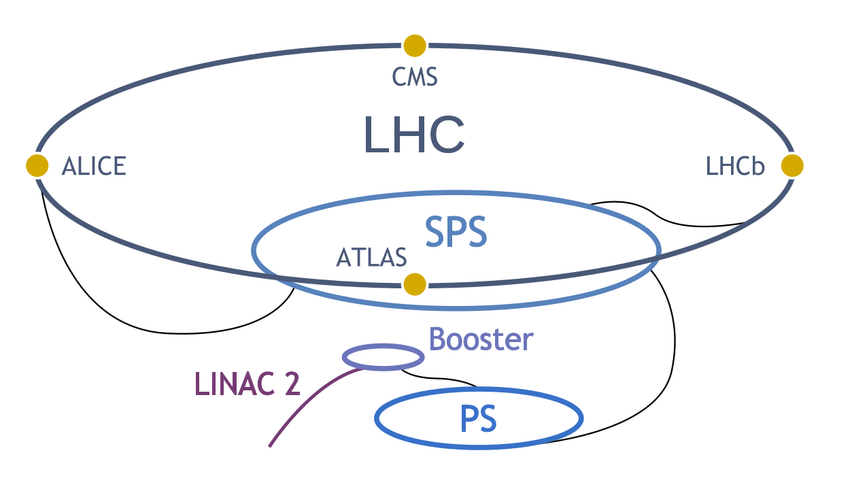
\includegraphics[width=\textwidth]{../ImmaginiTesi/LHC.png} 
  \end{minipage}
  \hfill 
  \begin{minipage}[b]{0.5\textwidth}
      \centering
      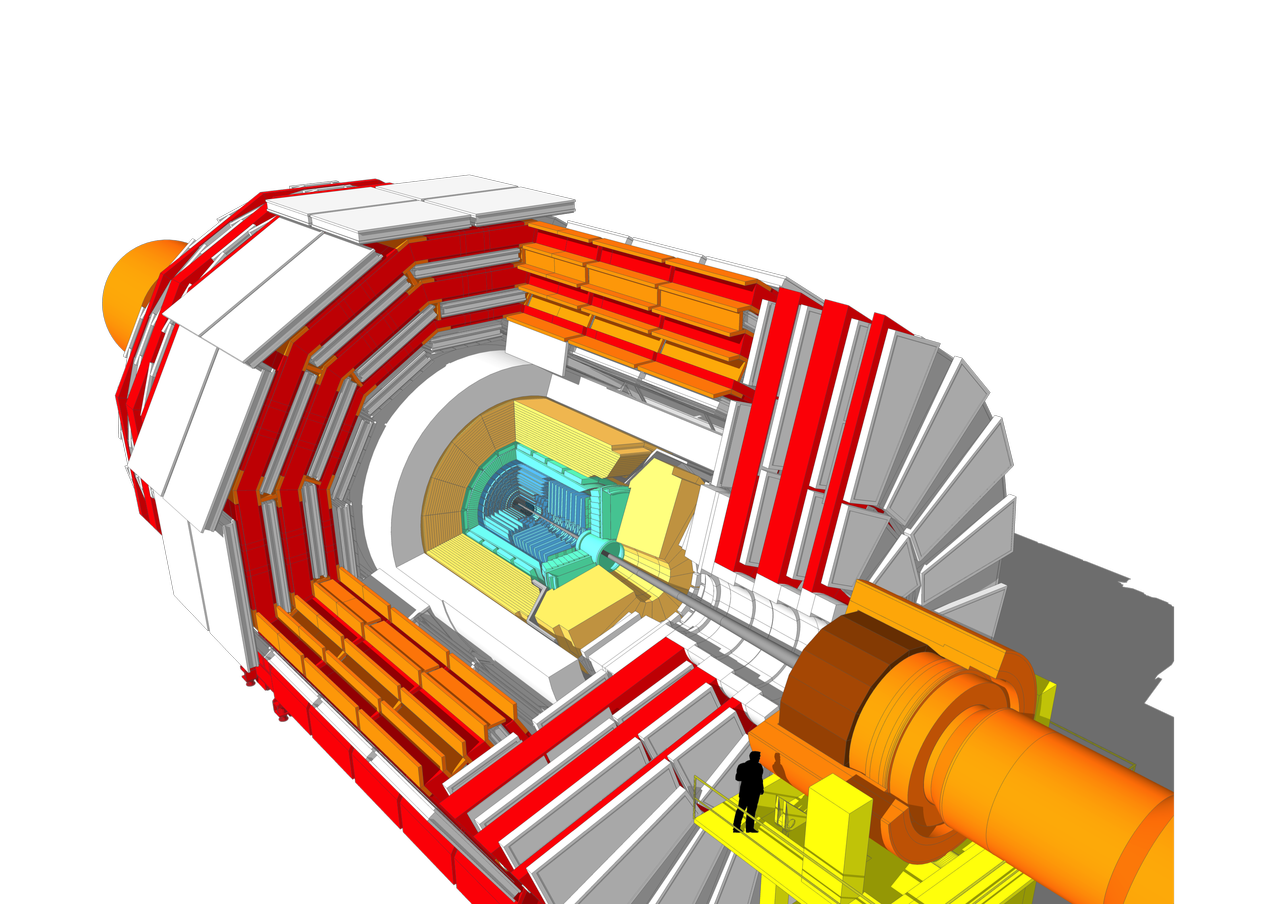
\includegraphics[width=\textwidth]{../ImmaginiTesi/CMS.png} 
  \end{minipage}
  \caption{Struttura dell'LHC e dei suoi rivelatori nei punti di interazione (sinistra), CMS (destra)}
  \label{fig:LHC-CMS}
\end{figure}

I protoni subiscono una serie di fasi di accelerazione prima di essere immessi nell'LHC \cite{evans2008lhc}: una prima fase di accelerazione fino a 50MeV ad opera di un acceleratore lineare Linac, poi vengono accelerati fino a 1.4GeV dal Proton Synchrotron Booster (PSB), quindi a 28GeV dal Proton Synchrotron (PS) e infine dal Super Proton Synchrotron (SPS) a 450GeV. A questo punto i protoni sono iniettati nell'LHC dove verranno accelerati fino a 7 TeV, collidendo frontalmente nei punti di interazione con una energia nel centro di massa $\sqrt{s} \approx 14$TeV.

L'LHC alterna periodi di fasi di attività e di raccolta dati (Run) con fasi di arresto in cui vengono effettuate opere di upgrade e di manutenzione. Tra la Run 1, iniziata nel 2009 e finita nel 2013, e la Run 2, tra 2015 e 2018, il sistema di trigger Level-1 (L1T) del CMS ha subito importanti miglioramenti (\textit{Phase 1}) rimpiazzando e potenziando hardware, elettronica e software del trigger permettendo, durante la Run 2, un incremento dell'energia di collisione protone protone nel centro di massa da 8 a 14 TeV \cite{sirunyan2020performance}. E' in programma nel 2025 un ulteriore upgrade dell'LHC (\textit{Phase 2}) che porterà un incremento della luminosità istantanea fino a $5\times 10^{34}$ \si{cm^{-2} s^{-1}}, aumentando quindi il numero di collisioni medio per BX da 50 a 140 \cite{collaboration2021phase}. In contemporanea, al fine di sfruttare appieno l'incremento della luminosità dell'LHC della Phase 2 (noto come \textit{HL-LHC}, High Luminosity LHC), è previsto un upgrade anche del sistema di detector del CMS, ed in particolare sul sistema di trigger L1, di cui parleremo nelle prossime sezioni.

\section{Compact Muon Solenoid}

Il rivelatore CMS è formato da un corpo cilindrico di 15 m di diametro e 21.6 m di lunghezza, per un peso di circa 14.000 tonnellate \cite{MasterThesisNicLai}. Locato nel punto di interazione IP5 in Cessy, Francia, il programma di fisica del CMS comprende vari ambiti nella fisica delle alte energie: dopo la scoperta del bosone di Higgs, nel 2012 e delle sue validazioni sperimentali compatibili con il modello standard (SM), lo studio di particelle esotiche e supersimmetriche sono di fondamentale importanza al CMS per la ricerca di Nuova Fisica, ovvero eventi non predetti dalle attuali teorie. Al fine di identificare questi eventi è necessario un sistema di trigger molto performante \cite{sirunyan2020performance} e a questo scopo in gioco il nuovo sistema di trigger che verrà implementato nella \textit{Phase 2}, che permetterà quindi di osservare fenomeni esotici con una risoluzione migliore (assieme ad un nuovo sistema di analisi dati, \textit{Data Scounting}, di cui discuteremo maggiormente dopo aver introdotto il sistema di trigger del CMS (??))

Di seguito una panoramica della struttura del CMS, dalle componenti più interne fino a quelle più esterne (Figura \ref{fig:LHC-CMS}):

\begin{itemize}
  \item 
\end{itemize}









\begin{comment}
\begin{figure}[t]
  \centering
  \begin{minipage}[b]{0.45\textwidth}
      \centering
      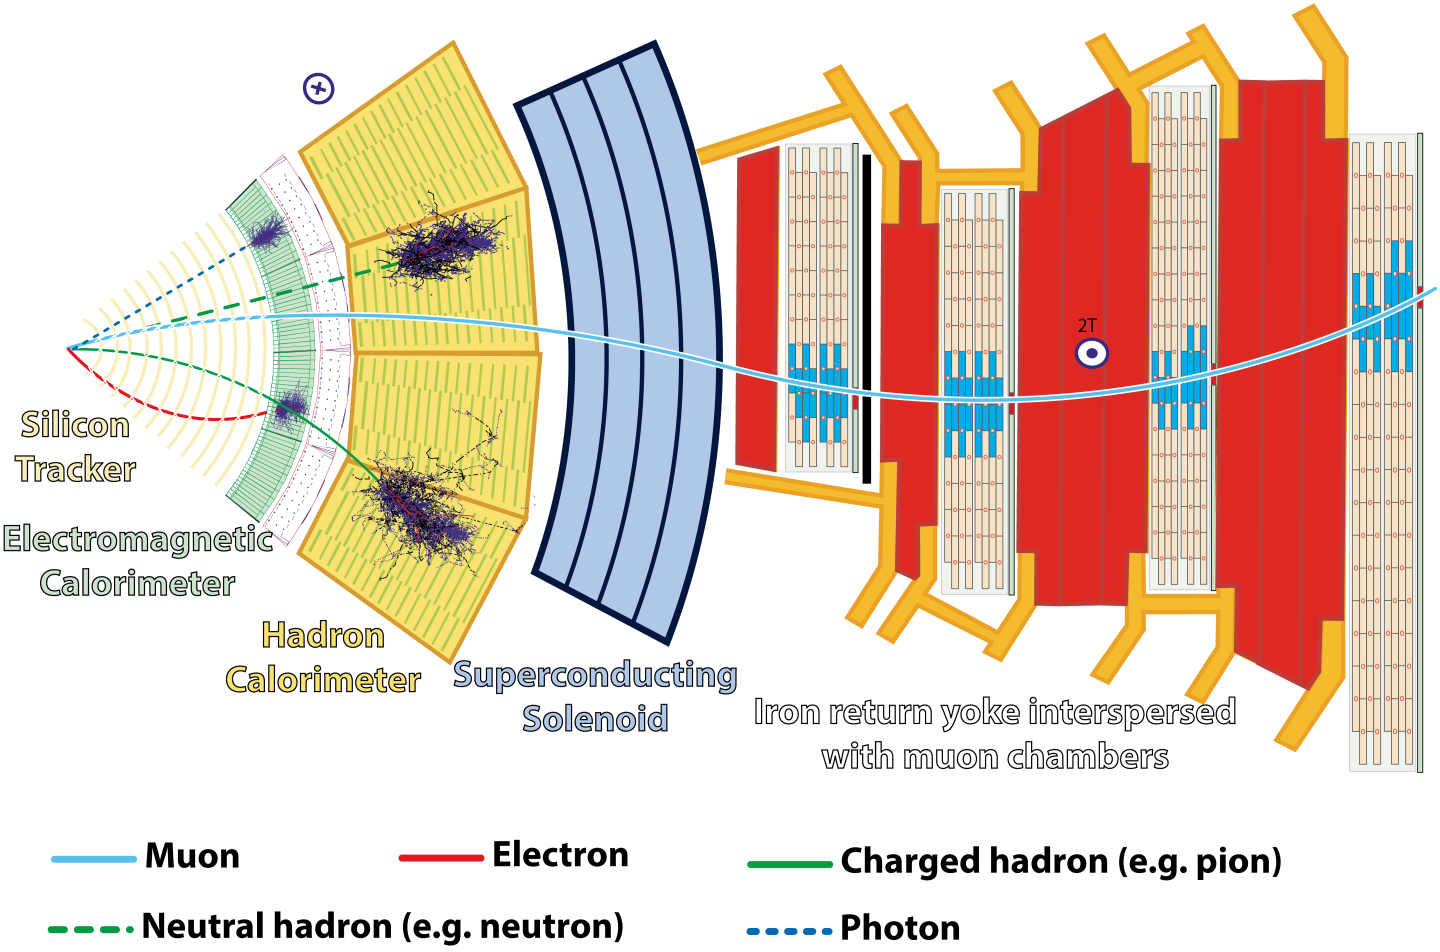
\includegraphics[width=\textwidth]{../ImmaginiTesi/CMS slice.png} 
  \end{minipage}
  \hfill 
  \begin{minipage}[b]{0.45\textwidth}
      \centering
      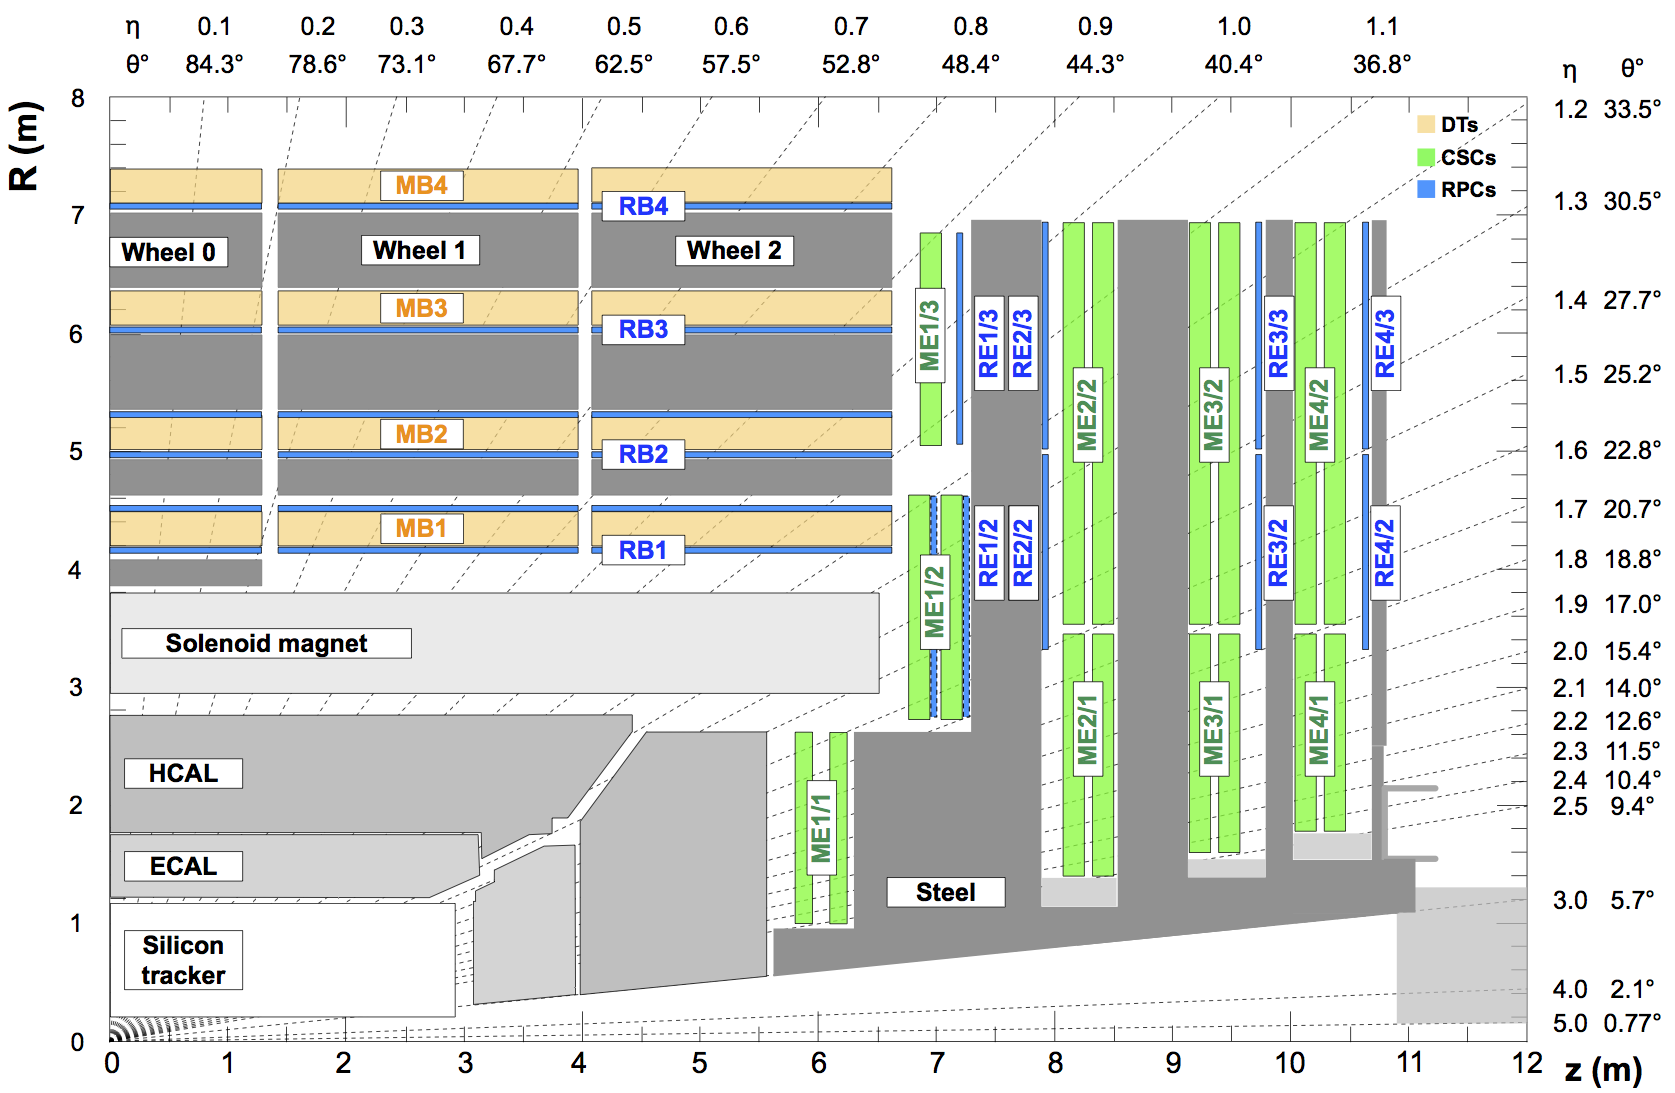
\includegraphics[width=\textwidth]{../ImmaginiTesi/CMSEtaView.png} 
  \end{minipage}
  \caption{Settore di CMS comprendente tutte le componenti (sinistra), vista nella variabile $\eta$ di CMS}
  \label{fig:SectorEtaView}
\end{figure}
\end{comment}












